\documentclass[11pt,a4paper]{ivoa}
\input tthdefs

\usepackage[utf8]{inputenc}
\usepackage{tabularx}
\usepackage{mathtools}

\title{Astronomical Data Query Language}

\ivoagroup{Data Access Layer Working Group}

\author[http://wiki.ivoa.net/twiki/bin/view/IVOA/IvoaVOQL]{The IVOA Virtual Observatory Query Language (VOQL) working group members}
\author[http://wiki.ivoa.net/twiki/bin/view/IVOA/IvoaDAL]{The IVOA Data Access Layer (DAL) working group members}

\editor[http://wiki.ivoa.net/twiki/bin/view/IVOA/DaveMorris]{Dave Morris}

\previousversion[http://www.ivoa.net/Documents/ADQL/2.0]{ADQL-2.0}

\begin{document}

\begin{abstract}
This document describes the Astronomical Data Query Language (ADQL).
ADQL has been developed based on SQL92.
This document describes the subset of the SQL grammar supported by ADQL.
Special restrictions and extensions to SQL92 have been defined in order
to support generic and astronomy specific operations.
\end{abstract}

\section*{Acknowledgments}

The authors would like to acknowledge all contributors to this and previous 
versions of this standard, especially:
P. Dowler,
J. Lusted,
M. A. Nieto-Santisteban,
W. O'Mullane,
M. Ohishi,
I. Ortiz,
P. Osuna,
Y Shirasaki,
and
A. Szalay.

\section*{Conformance-related definitions}

The words ``MUST'', ``SHALL'', ``SHOULD'', ``MAY'', ``RECOMMENDED'', and
``OPTIONAL'' (in upper or lower case) used in this document are to be
interpreted as described in IETF standard, \citet{std:RFC2119}.

The \emph{Virtual Observatory (VO)} is general term for a collection of
federated resources that can be used to conduct astronomical research,
education, and outreach. The \href{http://www.ivoa.net}{International Virtual
Observatory Alliance (IVOA)} is a global collaboration of separately funded
projects to develop standards and infrastructure that enable VO applications.

\section{Introduction}

The Astronomical Data Query Language (ADQL) is the language used by the
International Virtual Observatory Alliance (IVOA) to represent astronomy
queries posted to VO services. The IVOA has developed several standardized
protocols to access astronomical data, e.g., SIAP and SSAP for image and
spectral data respectively. These protocols might be satisfied using a single
table query. However, different VO services have different needs in terms
of query complexity and ADQL arises in this context.

The ADQL specification makes no distinction between core and advanced or
extended functionalities. Hence ADQL has been built according to a single
language definition (BNF based [1]). Any service making use of ADQL would
then define the level of compliancy to the language. This would allow the
notion of core and extension to be service-driven and it would decouple the
language from the service specifications.

ADQL is based on the Structured Query Language (SQL), especially on SQL 92. The
VO has a number of tabular data sets and many of them are stored in relational
databases, making SQL a convenient access means. A subset of the SQL grammar
has been extended to support queries that are specific to astronomy. Similarly
to SQL, the ADQL language definition is not semantically safe by design and
therefore this specification defines syntactical correctness only. Type safety
has been achieved as far as it can be done in SQL. The exact meaning of key
words indicating requirement levels can be found in the References section [2].

\subsection{Role within the VO Architecture}

\begin{figure}
\centering
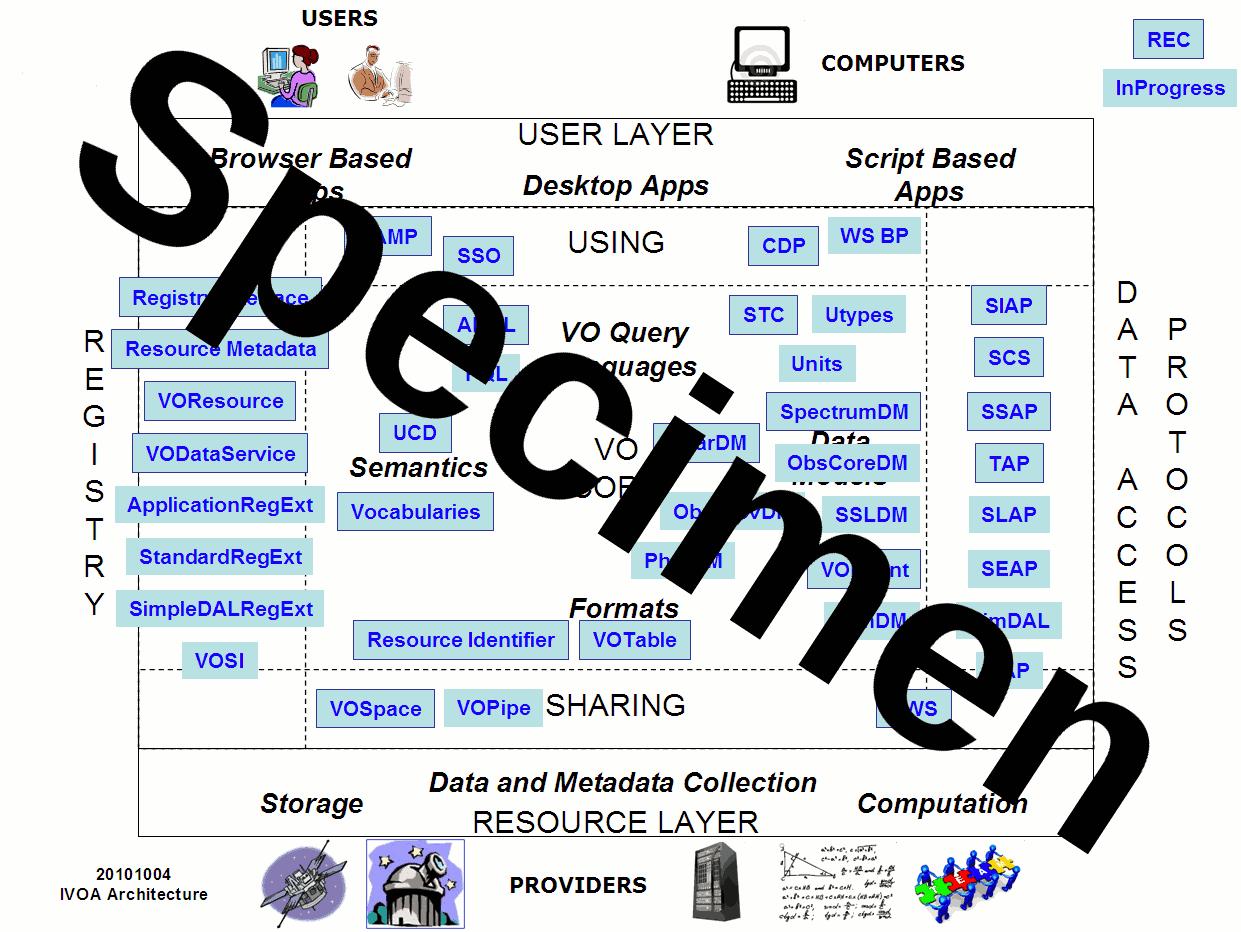
\includegraphics[width=0.9\textwidth]{archdiag.png}
\caption{Architecture diagram for this document}
\label{fig:archdiag}
\end{figure}

Fig.~\ref{fig:archdiag} shows the role this document plays within the
IVOA architecture \citep{note:VOARCH}.

\section{Astronomical Data Query Language (ADQL)}

This section describes the ADQL language specification. We will define in
subsequent sections the syntax for the special characters, reserved and non-
reserved words, identifiers and literals and then, finally, the syntax for
the query expression.

The formal notation for syntax of computing languages is often expressed
in the “Backus Naur Form” BNF. This syntax is used by popular tools for
producing parsers. Appendix A to this document provides the full BNF grammar
for ADQL. The following conventions are used through this document:

\begin{itemize}
\item Optional items are enclosed in meta symbols \verb:[: and \verb:]:
\item A group of items is enclosed in meta symbols \verb:{: and \verb:}:
\item Repetitive item (zero or more times) are followed by \verb:...:
\item Terminal symbols are enclosed by \verb:<: and \verb:>:
\item Terminals of meta-symbol characters (\verb:=,[,],(,),<,>,*:) are surrounded by quotes (\verb:“:) to distinguish them from meta-symbols
\item Case insensitiveness otherwise stated
\end{itemize}

\subsection{Characters, Keywords, Identifiers and Literals}
\subsubsection{Characters}

The language allows simple Latin letters (lower and upper case, i.e.
\verb:{aA-zZ}):, digits (\verb:{0-9}:) and the following special characters:

\begin{itemize}
\item space
\item single quote (\verb:’:)
\item double quote (\verb:“:)
\item percent (\verb:%:)
\item left and right parenthesis
\item asterisk (\verb:*:)
\item plus sign (\verb:+:)
\item minus sign (\verb:-:)
\item comma (\verb:,:)
\item period (\verb:.:)
\item solidus (\verb:/:)
\item colon (\verb.:.)
\item semicolon (\verb:;:)
\item less than operator (\verb:<:)
\item equals operator (\verb:=:)
\item greater than operator (\verb:>:)
\item underscore (\verb:_:)
\item ampersand (\verb:&:)
\item question mark (\verb:?:)
\item vertical bar (\verb:|:)
\end{itemize}

\subsubsection{Keywords and Identifiers}

Besides the character set, the language provides a list of reserved keywords
plus the syntax description for regular identifiers.

A reserved keyword has a special meaning in ADQL and cannot be used as
an identifier. These keywords must be enforced and should be extensive as
an escaping mechanism is already in place. We can extend the list of SQL92
reserved keywords to accommodate those useful for astronomical purposes and/or
present in a subset of vendor specific languages only (e.g. TOP). This leads
to the following list:

\begin{itemize}
\item SQL reserved keywords:
\end{itemize}

\begin{verbatim}
ABSOLUTE, ACTION, ADD, ALL, ALLOCATE, ALTER, AND, ANY, ARE, AS, ASC,
ASSERTION, AT, AUTHORIZATION, AVG, BEGIN, BETWEEN, BIT, BIT_LENGTH,
BOTH, BY, CASCADE, CASCADED, CASE, CAST, CATALOG, CHAR, CHARACTER,
CHARACTER_LENGTH, CHAR_LENGTH, CHECK, CLOSE, COALESCE, COLLATE,
COLLATION, COLUMN, COMMIT, CONNECT, CONNECTION, CONSTRAINT,
CONSTRAINTS, CONTINUE, CONVERT, CORRESPONDING, COUNT, CREATE,
CROSS, CURRENT, CURRENT_DATE, CURRENT_TIME, CURRENT_TIMESTAMP,
CURRENT_USER, CURSOR, DATE, DAY, DEALLOCATE, DECIMAL, DECLARE,
DEFAULT, DEFERRABLE, DEFERRED, DELETE, DESC, DESCRIBE, DESCRIPTOR,
DIAGNOSTICS, DISCONNECT, DISTINCT, DOMAIN, DOUBLE, DROP, ELSE, END,
END-EXEC, ESCAPE, EXCEPT, EXCEPTION, EXEC, EXECUTE, EXISTS, EXTERNAL,
EXTRACT, FALSE, FETCH, FIRST, FLOAT, FOR, FOREIGN, FOUND, FROM,
FULL, GET, GLOBAL, GO, GOTO, GRANT, GROUP, HAVING, HOUR, IDENTITY,
IMMEDIATE, IN, INDICATOR, INITIALLY, INNER, INPUT, INSENSITIVE,
INSERT, INT, INTEGER, INTERSECT, INTERVAL, INTO, IS, ISOLATION,
JOIN, KEY, LANGUAGE, LAST, LEADING, LEFT, LEVEL, LIKE, LOCAL, LOWER,
MATCH, MAX, MIN, MINUTE, MODULE, MONTH, NAMES, NATIONAL, NATURAL,
NCHAR, NEXT, NO, NOT, NULL, NULLIF, NUMERIC, OCTET_LENGTH, OF, ON,
ONLY, OPEN, OPTION, OR, ORDER, OUTER, OUTPUT, OVERLAPS, PAD, PARTIAL,
POSITION, PRECISION, PREPARE, PRESERVE, PRIMARY, PRIOR, PRIVILEGES,
PROCEDURE, PUBLIC, READ, REAL, REFERENCES, RELATIVE, RESTRICT,
REVOKE, RIGHT, ROLLBACK, ROWS, SCHEMA, SCROLL, SECOND, SECTION,
SELECT, SESSION, SESSION_USER, SET, SIZE, SMALLINT, SOME, SPACE, SQL,
SQLCODE, SQLERROR, SQLSTATE, SUBSTRING, SUM, SYSTEM_USER, TABLE,
TEMPORARY, THEN, TIME, TIMESTAMP, TIMEZONE_HOUR, TIMEZONE_MINUTE,
TO, TRAILING, TRANSACTION, TRANSLATE, TRANSLATION, TRIM, TRUE,
UNION, UNIQUE, UNKNOWN, UPDATE, UPPER, USAGE, USER, USING, VALUE,
VALUES, VARCHAR, VARYING, VIEW, WHEN, WHENEVER, WHERE, WITH, WORK,
WRITE, YEAR, ZONE
\end{verbatim}

\begin{itemize}
\item ADQL reserved keywords:
\end{itemize}

\begin{verbatim}
ABS, ACOS, ASIN, ATAN, ATAN2, CEILING, COS, DEGREES, EXP, FLOOR,
LOG, LOG10, MOD, PI, POWER, RADIANS, RAND, ROUND, SIN, SQRT, TAN,
TOP, TRUNCATE
\end{verbatim}

The identifiers are used to express, for example, a table or a column
reference name.

Both the identifiers and the keywords are case insensitive. They SHALL
begin with a letter \verb:{aA-zZ}:. Subsequent characters shall be letters,
underscores or digits \verb:{0-9}: as follows:

\begin{verbatim}
    <Latin_letter> [{ <underscore> | {<Latin_letter> | <digit>} }]
\end{verbatim}

For practical purposes the language specification should be able to address
reserved keyword and special character conflicts. To do so the language
provides a way to escape a non-compliant identifier by using the double
quote character as a delimiter.

ADQL allows making use of the same quoting mechanism to handle the case
sensitiveness if needed.

\subsubsection{Literals}

Finally we define the syntax rules for the different data types: string and number. A string literal is a character expression delimited by single quotes. Literal numbers are expressed in BNF as follows:

\begin{verbatim}
    <unsigned_numeric_literal> ::=
        <exact_numeric_literal> | <approximate_numeric_literal>

    <exact_numeric_literal> ::=
        <unsigned_integer> [<period> [<unsigned_integer>]]
        | <period><unsigned_integer>

    <unsigned_integer> ::= <digit>...

    <approximate_numeric_literal> ::= <mantissa> E <exponent>

    <mantissa> ::= <exact_numeric_literal>

    <exponent> ::= <signed_integer>

    <signed_integer> ::= [<sign>] <unsigned_integer>

    <sign> ::= <plus_sign> | <minus_sign>
\end{verbatim}

Regarding the usage of other data types like datetime and timestamp, ADQL
can deal with them similarly to how SQL does: using the string literal
construct. As Relation Database Manager Systems (RDBMs) do, a service should
be able to implicitly convert strings to internal (datetime or timestamp)
form using a variety of techniques, where e.g. ISO 8601 is an acceptable
format. Therefore, as with other string representations, it should be up to
the service capability to understand such specific formats.

\subsection{Query syntax}

A full and complete syntax of the select statement can be found in “Appendix
A: BNF Grammar” at the \verb:<query_specification>: construct. Follows a simplified
syntax for the \verb:SELECT: statement showing the main constructs for the query
specification:

\begin{verbatim}
    SELECT
        [ ALL | DISTINCT ]
        [ TOP unsigned_integer ]
        {
             * |
             { value_expression [ [AS] column_name ] }, ...
         }
        FROM {
                {
                table_name [ [AS] identifier ] |
                ( SELECT ....) [ [AS] identifier ] |
                table_name [NATURAL]
                    [ INNER | { LEFT | RIGHT | FULL [OUTER] } ]
                    JOIN table_name
                    [ON search_condition | USING ( column_name,...) ]
                },
            ...
            }

        [ WHERE search_condition ]
        [ GROUP BY column_name, ... ]
        [ HAVING search_condition ]
        [ ORDER BY
            { column_name | unsigned_integer } [ ASC | DESC],
            ...
            ]
\end{verbatim}

The SELECT statement defines a query to some derived table(s) specified
in the FROM clause. As a result of this query, a subset of the table(s)
is returned. The order of the rows MAY be arbitrary unless ORDER BY clause
is specified. The order of the columns to return SHALL be the same as the
order specified in the selection list, or the order defined in the original
table if asterisk is specified. TOP n construct is used to return the first
n-rows. The selection list MAY include any numeric, string or geometry value
expression. In the following sections some constructs requiring further
description are presented.

\subsubsection{Table subqueries and Joins}

Table subqueries are present and can be used by some existing predicates
within the search condition (IN and BETWEEN most likely) or as an artifact
of building derived tables. Among the different types of join, ADQL supports
INNER and OUTER (LEFT, RIGHT and FULL) joins. If none is specified, the
default is INNER. All of these can be NATURAL or not. The join condition
does not support embedded sub joins.

\subsubsection{Search condition}

The search condition can be part of several other clauses: JOIN, HAVING and,
obviously, WHERE. Standard logical operators are present in its description
(AND, OR and NOT). Five different types of predicates are present in which
different types of reserved keywords or characters are used:

\begin{itemize}
\item Standard comparison operators: \verb:=:, \verb:!=:, \verb:<>:, \verb:<:, \verb:>:, \verb:<=:, \verb:>=:
\item \verb:BETWEEN:
\item \verb:LIKE:
\item \verb:NULL:
\item \verb:EXISTS:
\end{itemize}

\subsection{Mathematical and Trigonometrical Functions}

ADQL declares a list of reserved keywords (section 2.1.2) which defines
a set of mathematical and trigonometrical function names. Their syntax,
usage and description are detailed in the following tables:

\begin{table}[thm]\footnotesize
    \begin{tabular}{|p{0.20\textwidth}|p{0.125\textwidth}|p{0.125\textwidth}|p{0.55\textwidth}|}
        \hline

        \hline
        \textbf{Name} &
        \textbf{Argument \newline data type} &
        \textbf{Return \newline data type} &
        \textbf{Description} \\

        \hline
        abs(x) &
        double&double &
        Returns the absolute value of x.\\

        \hline
        ceiling(x) &
        double&double &
        Returns the smallest double value that is not less than the argument x and is equal to a mathematical integer.\\

        \hline
        degrees(x) &
        double &
        double &
        Converts an angle to degrees. Argument x must be in radians.\\

        \hline
        exp(x) &
        double &
        double &
        Returns Euler’s number e raised to the power of x.\\

        \hline
        floor(x) &
        double &
        double &
        Returns the largest double value that is not greater than the argument x and is equal to a mathematical integer.\\

        \hline
        log(x) &
        double &
        double &
        Returns the natural logarithm (base e) of a double value. Value x must be greater than zero.\\
        
        \hline
        log10(x) &
        double &
        double &
        Returns the base 10 logarithm of a double value. Value x must be greater than zero.\\

        \hline
        mod(x, y) &
        double &
        double &
        Returns the remainder of y/x.\\
        
        \hline
        pi() &
        n/a &
        double &
        The \(\pi\) constant.\\
        
        \hline
        power(x, y) &
        x double \newline y double &
        double &
        Returns the value of the first argument raised to the power of the second argument.\\

        \hline
        radians(x) &
        double &
        double &
        Converts an angle to radians. Argument x must be in degrees.\\

        \hline
        sqrt(x) &
        double &
        double &
        Returns the positive square root of a double value.\\

        \hline
        rand(x) &
        integer &
        double &
        Returns a random value between 0.0 and 1.0, where x is a seed  value.\\

        \hline
        round(x, n) &
        x double \newline n integer &
        double &
        Rounds double value x to n number of decimal places, with the default being to round to the nearest integer.
        To round to the left of the decimal point, a negative number should be provided.\\

        \hline
        truncate(x, n) &
        x double \newline n integer &
        double &
        Returns the result of truncating the argument x to n decimal places.\\

        \hline
    \end{tabular}
    \caption{Mathematical functions}
    \label{table:extable}
\end{table}

\begin{table}[thm]\footnotesize
    \begin{tabular}{|p{0.20\textwidth}|p{0.125\textwidth}|p{0.125\textwidth}|p{0.55\textwidth}|}
        \hline

        \hline
        \textbf{Name} &
        \textbf{Argument \newline data type} &
        \textbf{Return \newline data type} &
        \textbf{Description} \\

        \hline
        acos(x) &
        double &
        double &
        Returns the arc cosine of an angle, in the range of 0 through \(\pi\) radians. Absolute value of x must be lower or equal than 1.0.\\

        \hline
        asin(x) &
        double &
        double &
        Returns the arc sine of an angle, in the range of -\(\pi\)/2 through \(\pi\)/2 radians. Absolute value of x must be and lower or equal than 1.0.\\

        \hline
        atan(x) &
        double &
        double &
        Returns the arc tangent of an angle, in the range of -\(\pi\)/2 through \(\pi\)/2 radians.\\
        
        \hline
        atan2(y,x) &
        double &
        double &
        Converts rectangular coordinates x,y to polar angle. It computes the arc tangent of y/x in the range of –\(\pi\) through \(\pi\) radians.\\

        \hline
        cos(x) &
        double &
        double &
        Returns the cosine of an angle, in the range of -1.0 through 1.0. Argument x must be in radians.\\

        \hline
        sin(x) &
        double &
        double &
        Returns the sine of an angle, in the range of -1.0 through 1.0. Argument x must be in radians.\\

        \hline
        tan(x) &
        double &
        double &
        Returns the tangent of an angle. Argument x must be in radians.\\

        \hline
    \end{tabular}
    \caption{Trigonometrical functions}
    \label{table:extable}
\end{table}

\subsection{Geometrical Functions}
\subsubsection{Overview}

In addition to the mathematical functions, ADQL provides a set of geometrical
functions to enhance the astronomical usage of the language. The list of
ADQL reserved keywords shown in Section 2.1.2 is therefore extended with
the following function names:

\begin{verbatim}
AREA, BOX, CENTROID, CIRCLE, CONTAINS, COORD1, COORD2,
COORDSYS, DISTANCE, INTERSECTS, POINT, POLYGON, REGION
\end{verbatim}

A special attention has to be paid to the REGION function. As can be seen more
in detail in Section 2.4.14, this construct is a general purpose function and
it takes a string value expression as argument. The format of the string is
to be specified by a service that accepts ADQL by referring to a standard
format. Currently STC/s (See [3] and [4]) is the only standardized string
representation a service can declare.



\appendix

\section{Changes from Previous Versions}

\subsection{Changes from ADQL-2.0}




\bibliography{ivoatex/ivoabib}

\end{document}

